\section*{Randomly Generated Example}

The methods and metrics defined above are demonstrated using a vehicle on a randomly generated \gls{sng}. In this example, a \gls{sng} containing 15 locations and 85 stations distributed across a 1000 km square is generated with randomized node locations. Each location has a population of one million persons. Each station contains between 1 and 5 ports. Edges exist between all nodes and are assigned Pythagorean distances. All edges are assumed to be traversed at 105 kmh. The supply stations deliver an average of 45 kWh per vehicle at an average rate of 80 kW. The arrivals ratio is sampled from $N(1, 0.25)$ The vehicle used has a relatively low range of 262 km. Two drivers are modeled. A cautious driver is modeled using ($p_0 = 0.9$, $p_1 = 1.0$) and a aggressive driver is modeled using ($p_0 = 0$, $p_1 = 0.1$). Additionally port reliability at the stations is modeled as 75\% in a low reliability scenario and 95\% in a high reliability scenario.

\begin{figure}[H]
	\centering
	\begin{subfigure}[t]{.5\linewidth}
		\centering\captionsetup{width = .8\linewidth}
		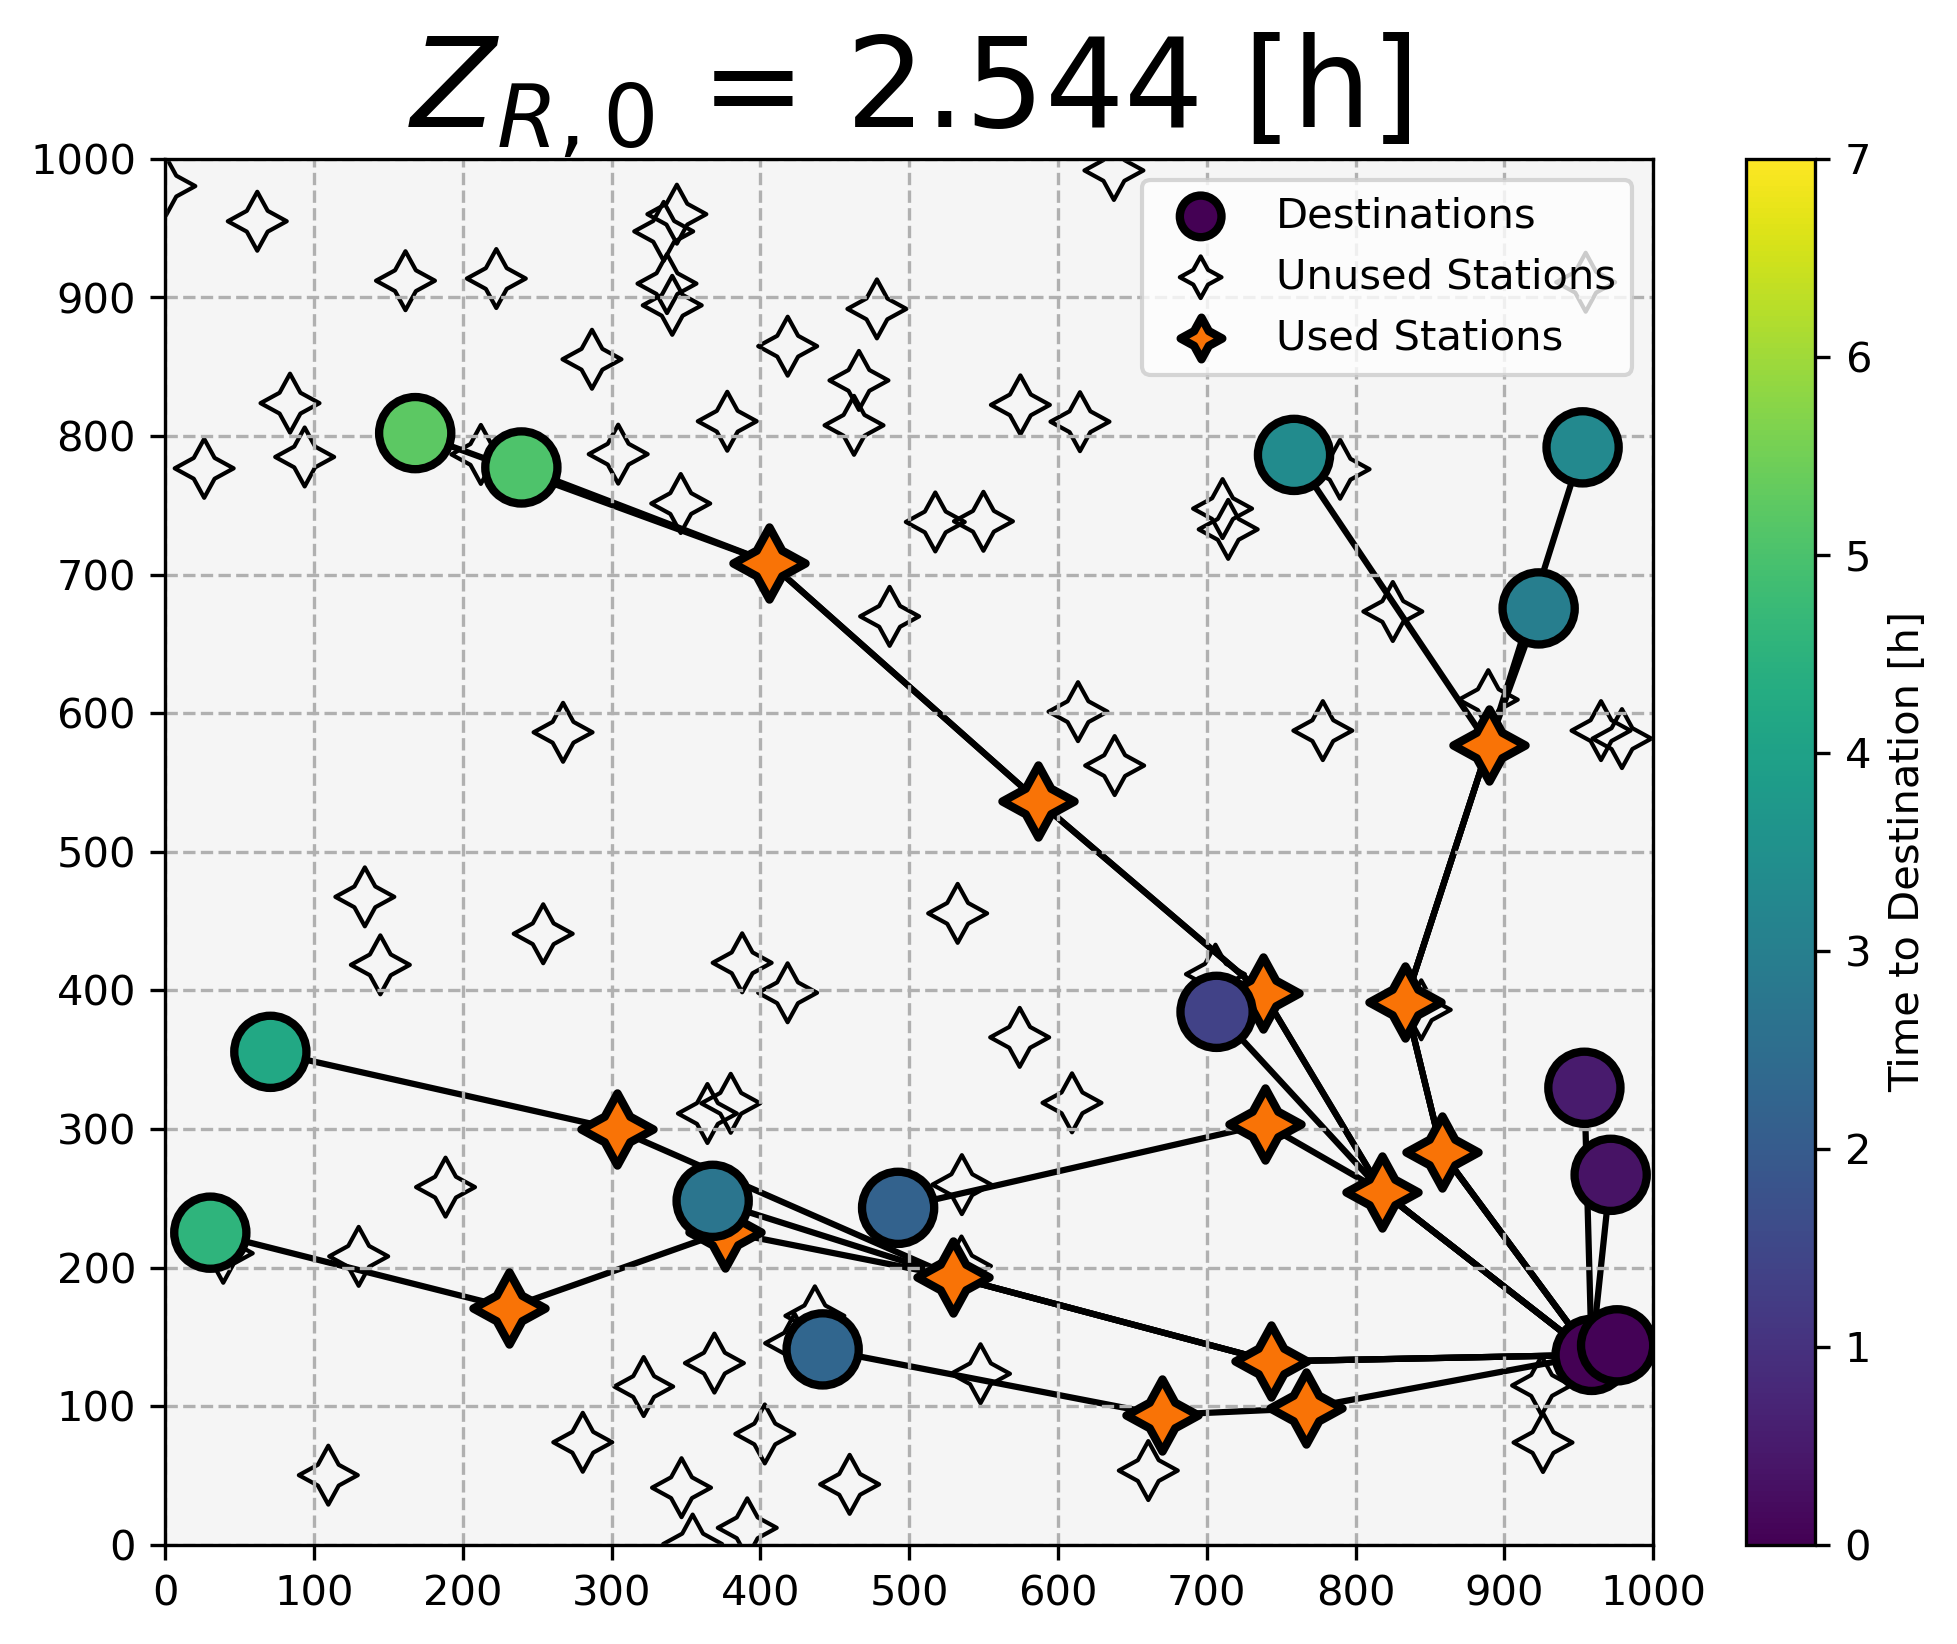
\includegraphics[width = \linewidth]{figs/random_example_high_reliability_aggressive_perceived.png}
		\caption{High reliability, aggressive}
	\end{subfigure}%
	\begin{subfigure}[t]{.5\linewidth}
		\centering\captionsetup{width = .8\linewidth}
		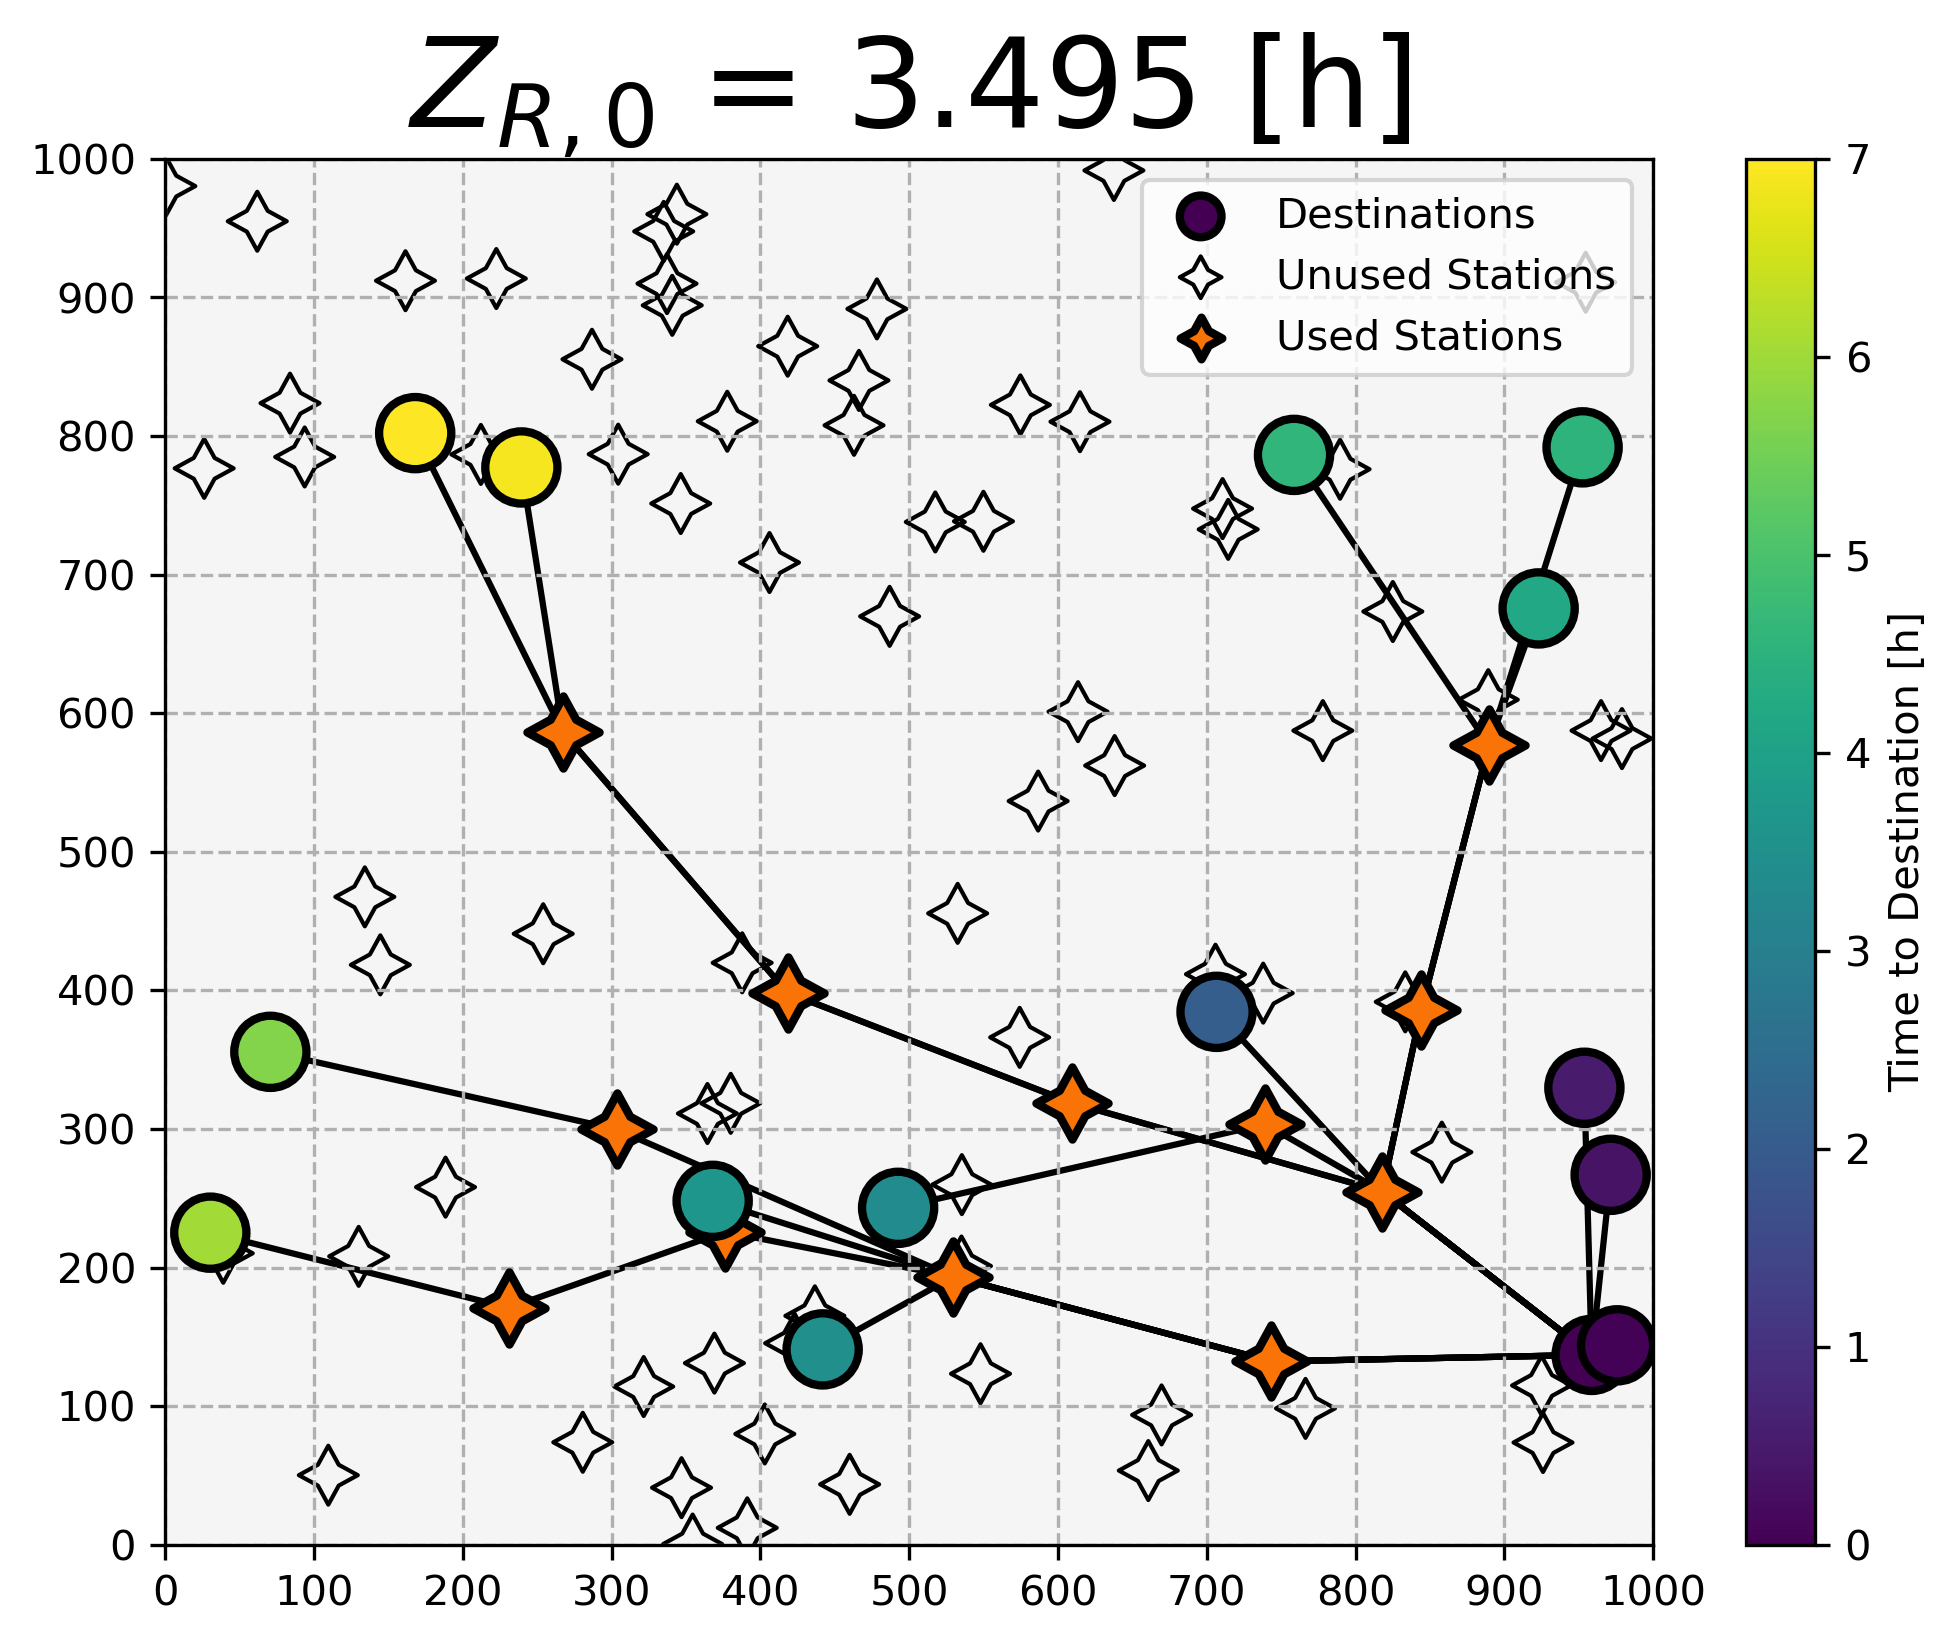
\includegraphics[width = \linewidth]{figs/random_example_high_reliability_cautious_perceived.png}
		\caption{High reliability, cautious}
	\end{subfigure}
	\begin{subfigure}[t]{.5\linewidth}
		\centering\captionsetup{width = .8\linewidth}
		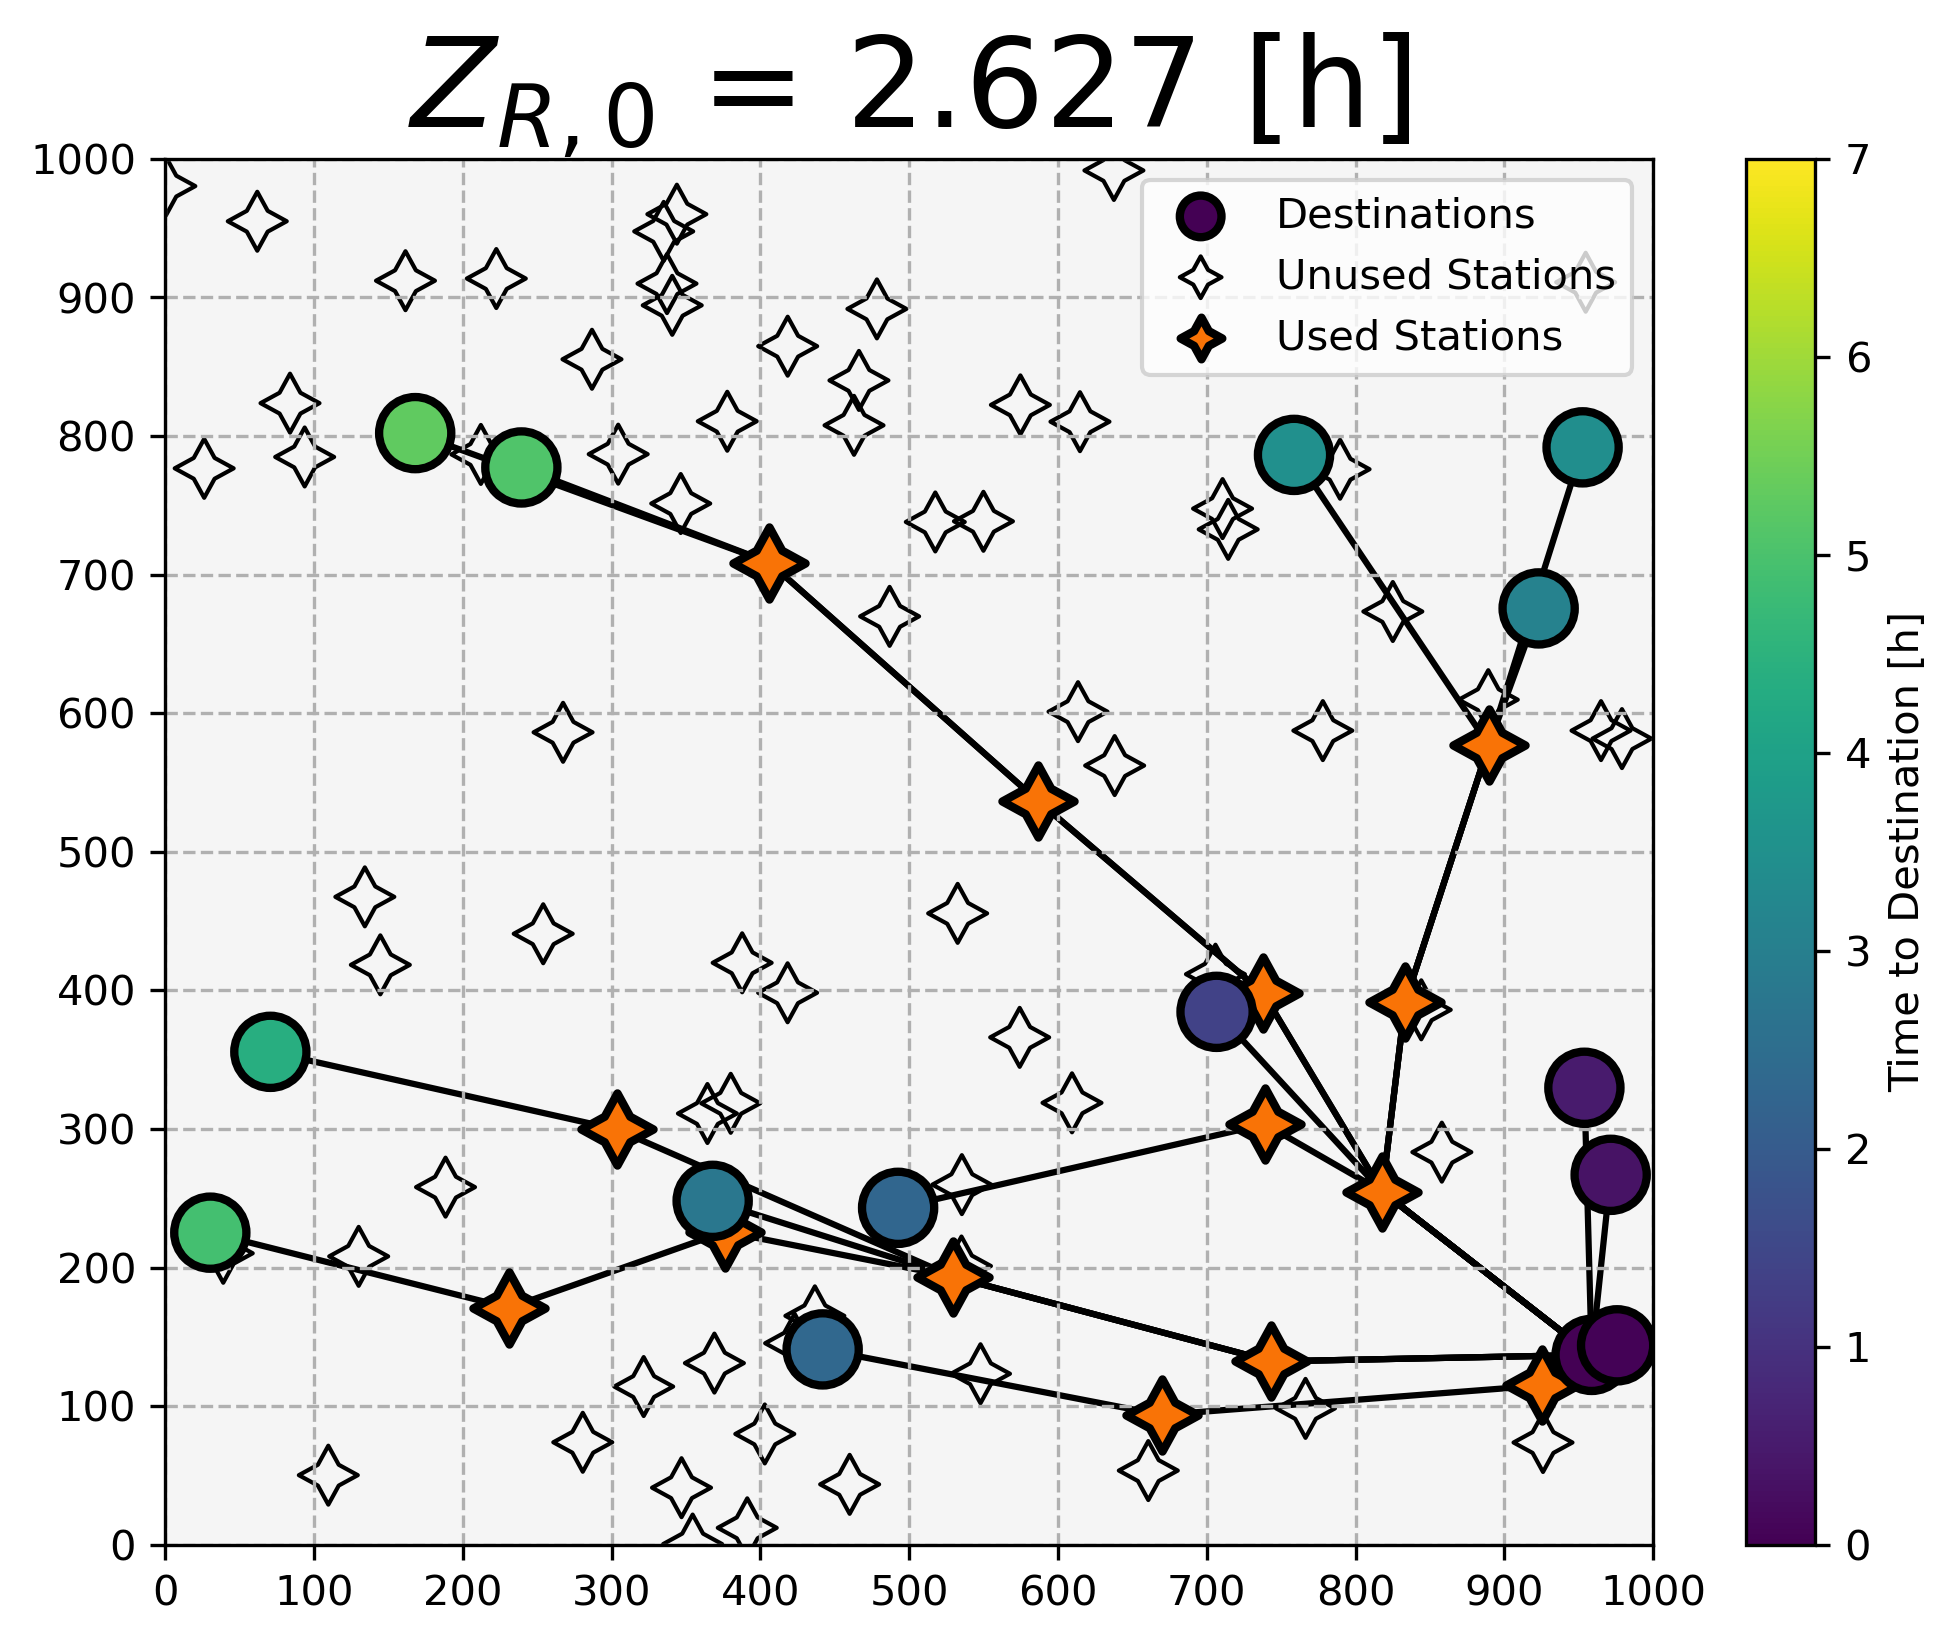
\includegraphics[width = \linewidth]{figs/random_example_low_reliability_aggressive_perceived.png}
		\caption{Low reliability, aggressive}
	\end{subfigure}%
	\begin{subfigure}[t]{.5\linewidth}
		\centering\captionsetup{width = .8\linewidth}
		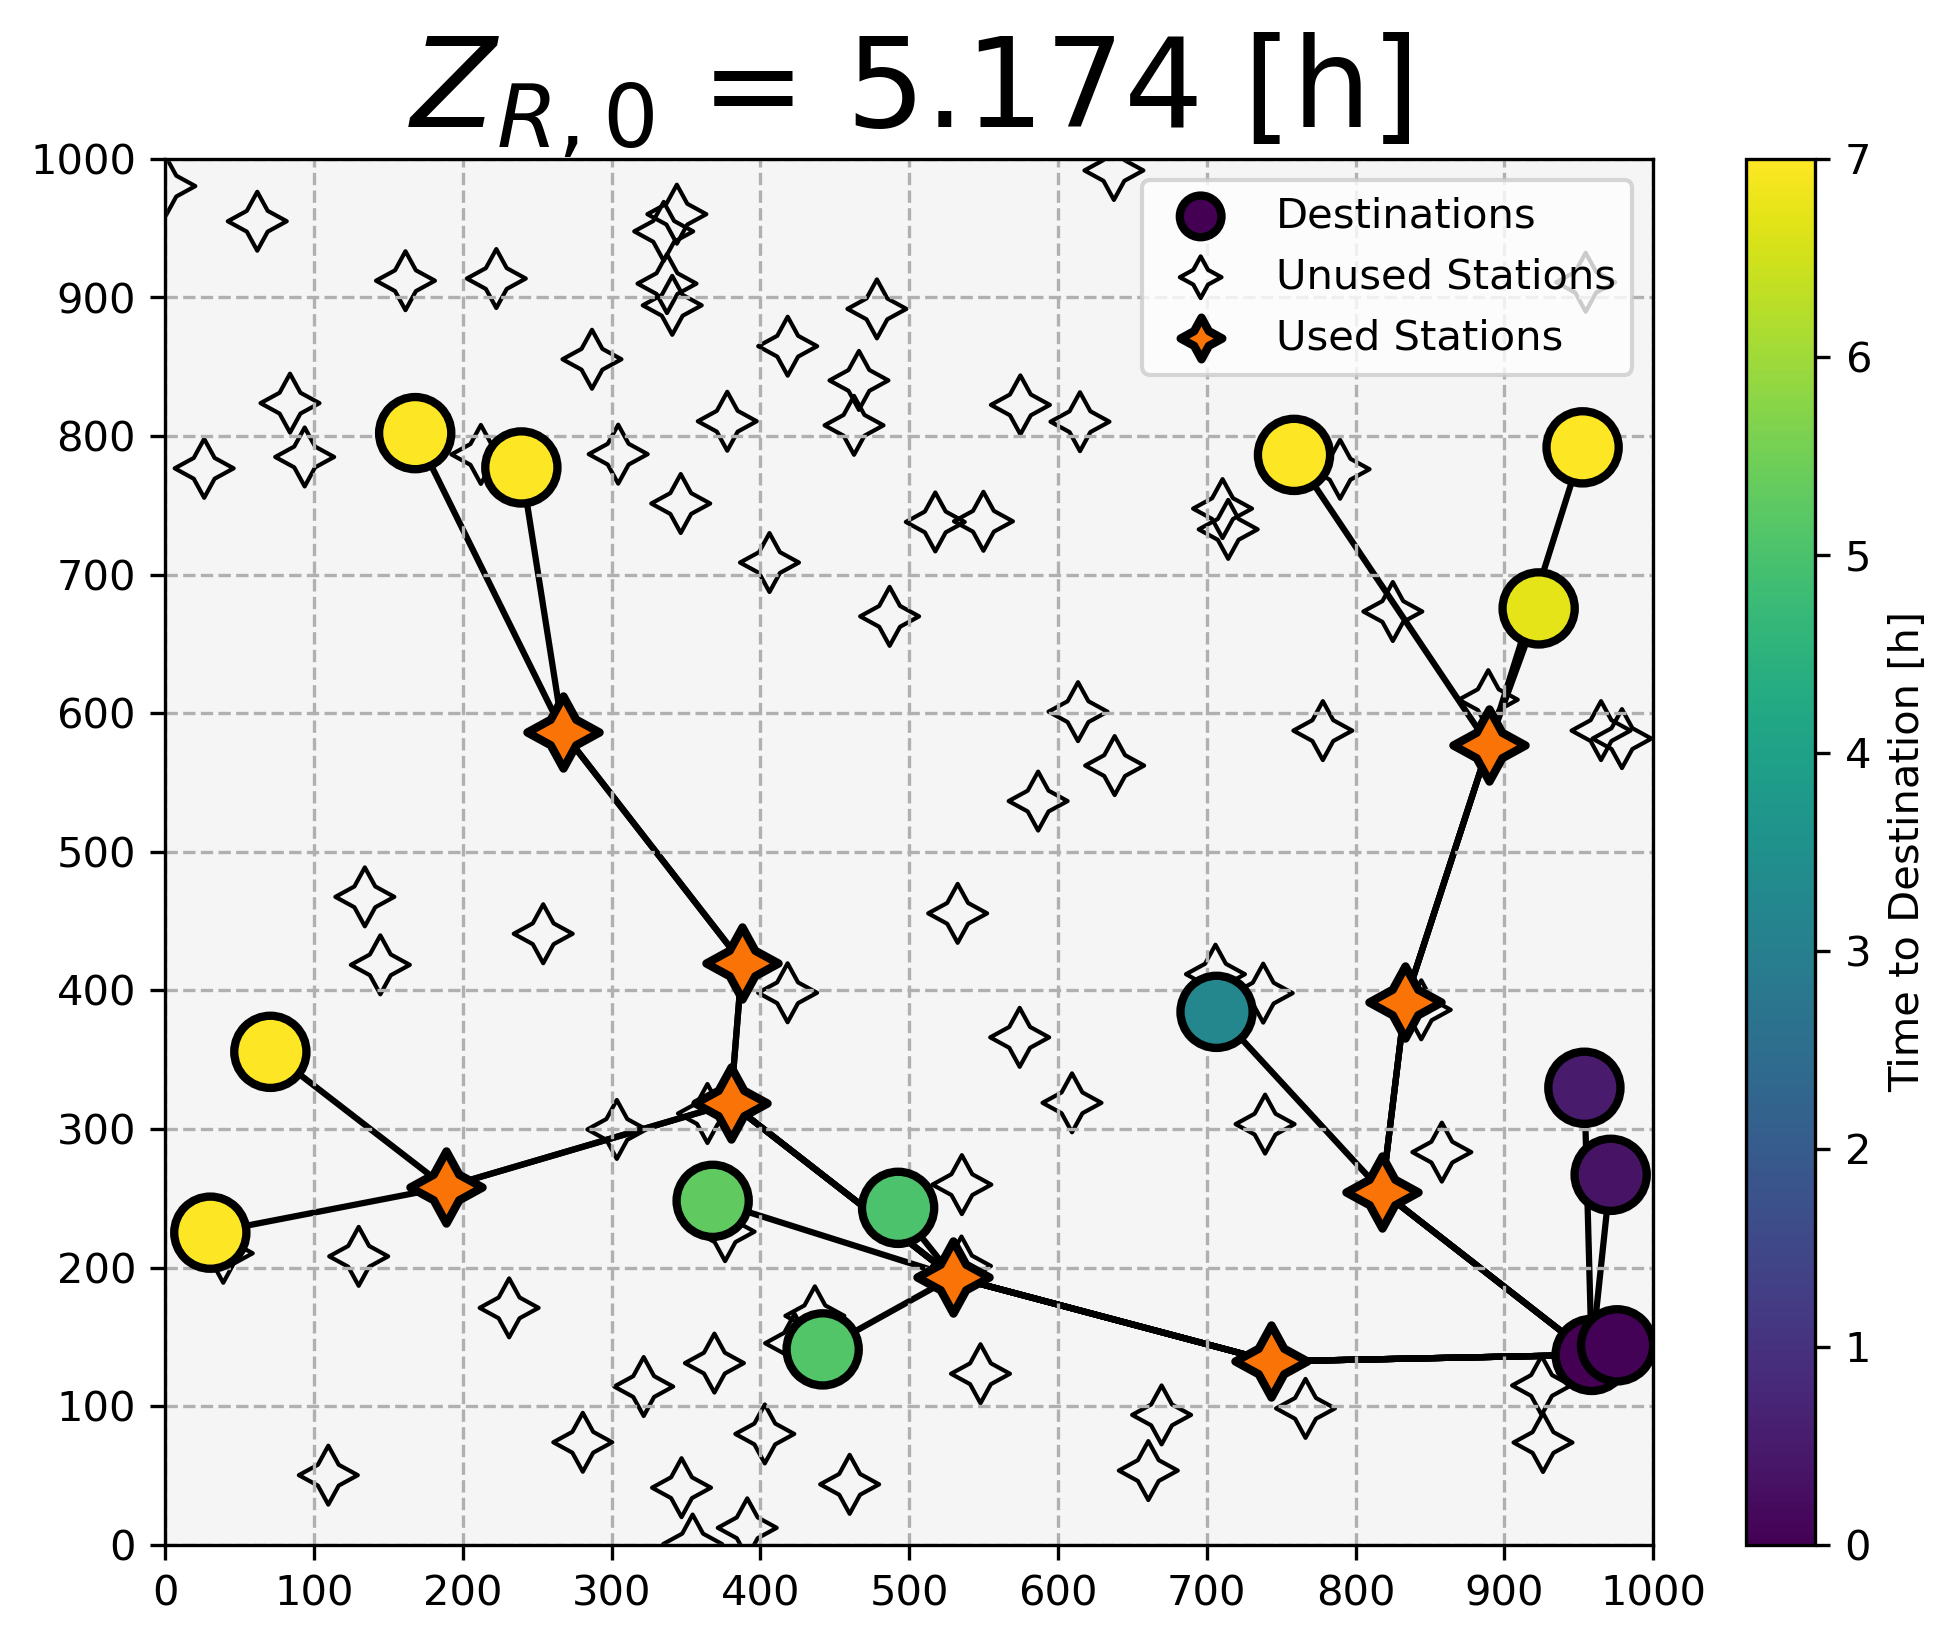
\includegraphics[width = \linewidth]{figs/random_example_low_reliability_cautious_perceived.png}
		\caption{Low reliability, cautious}
	\end{subfigure}
	\caption{Perceived Specific Regional Impedance by risk attitude and port reliability.}
	\label{fig:perceived_srta_random_perceived}
\end{figure}

The scenarios presented in Figure \ref{fig:perceived_srta_random_perceived} consider Specific Regional Impedance as perceived by the driver. The aggressive driver is only concerned with the best 10\% of outcomes where the cautious driver is only concerned with the worst 10\% of outcomes. The differences in perceived costs-to-travel are quite stark between the aggressive and cautious driver in both cases but this difference is larger when reliability is low. Drivers may operate off of perception but a regional transportation authority may be more concerned with mean outcomes. The neutral expectations ($p_0 = 0$, $p_1 = 1$) of the routes taken by the drivers are shown in Figure \ref{fig:perceived_srta_random_actual}.

\begin{figure}[H]
	\centering
	\begin{subfigure}[t]{.5\linewidth}
		\centering\captionsetup{width = .8\linewidth}
		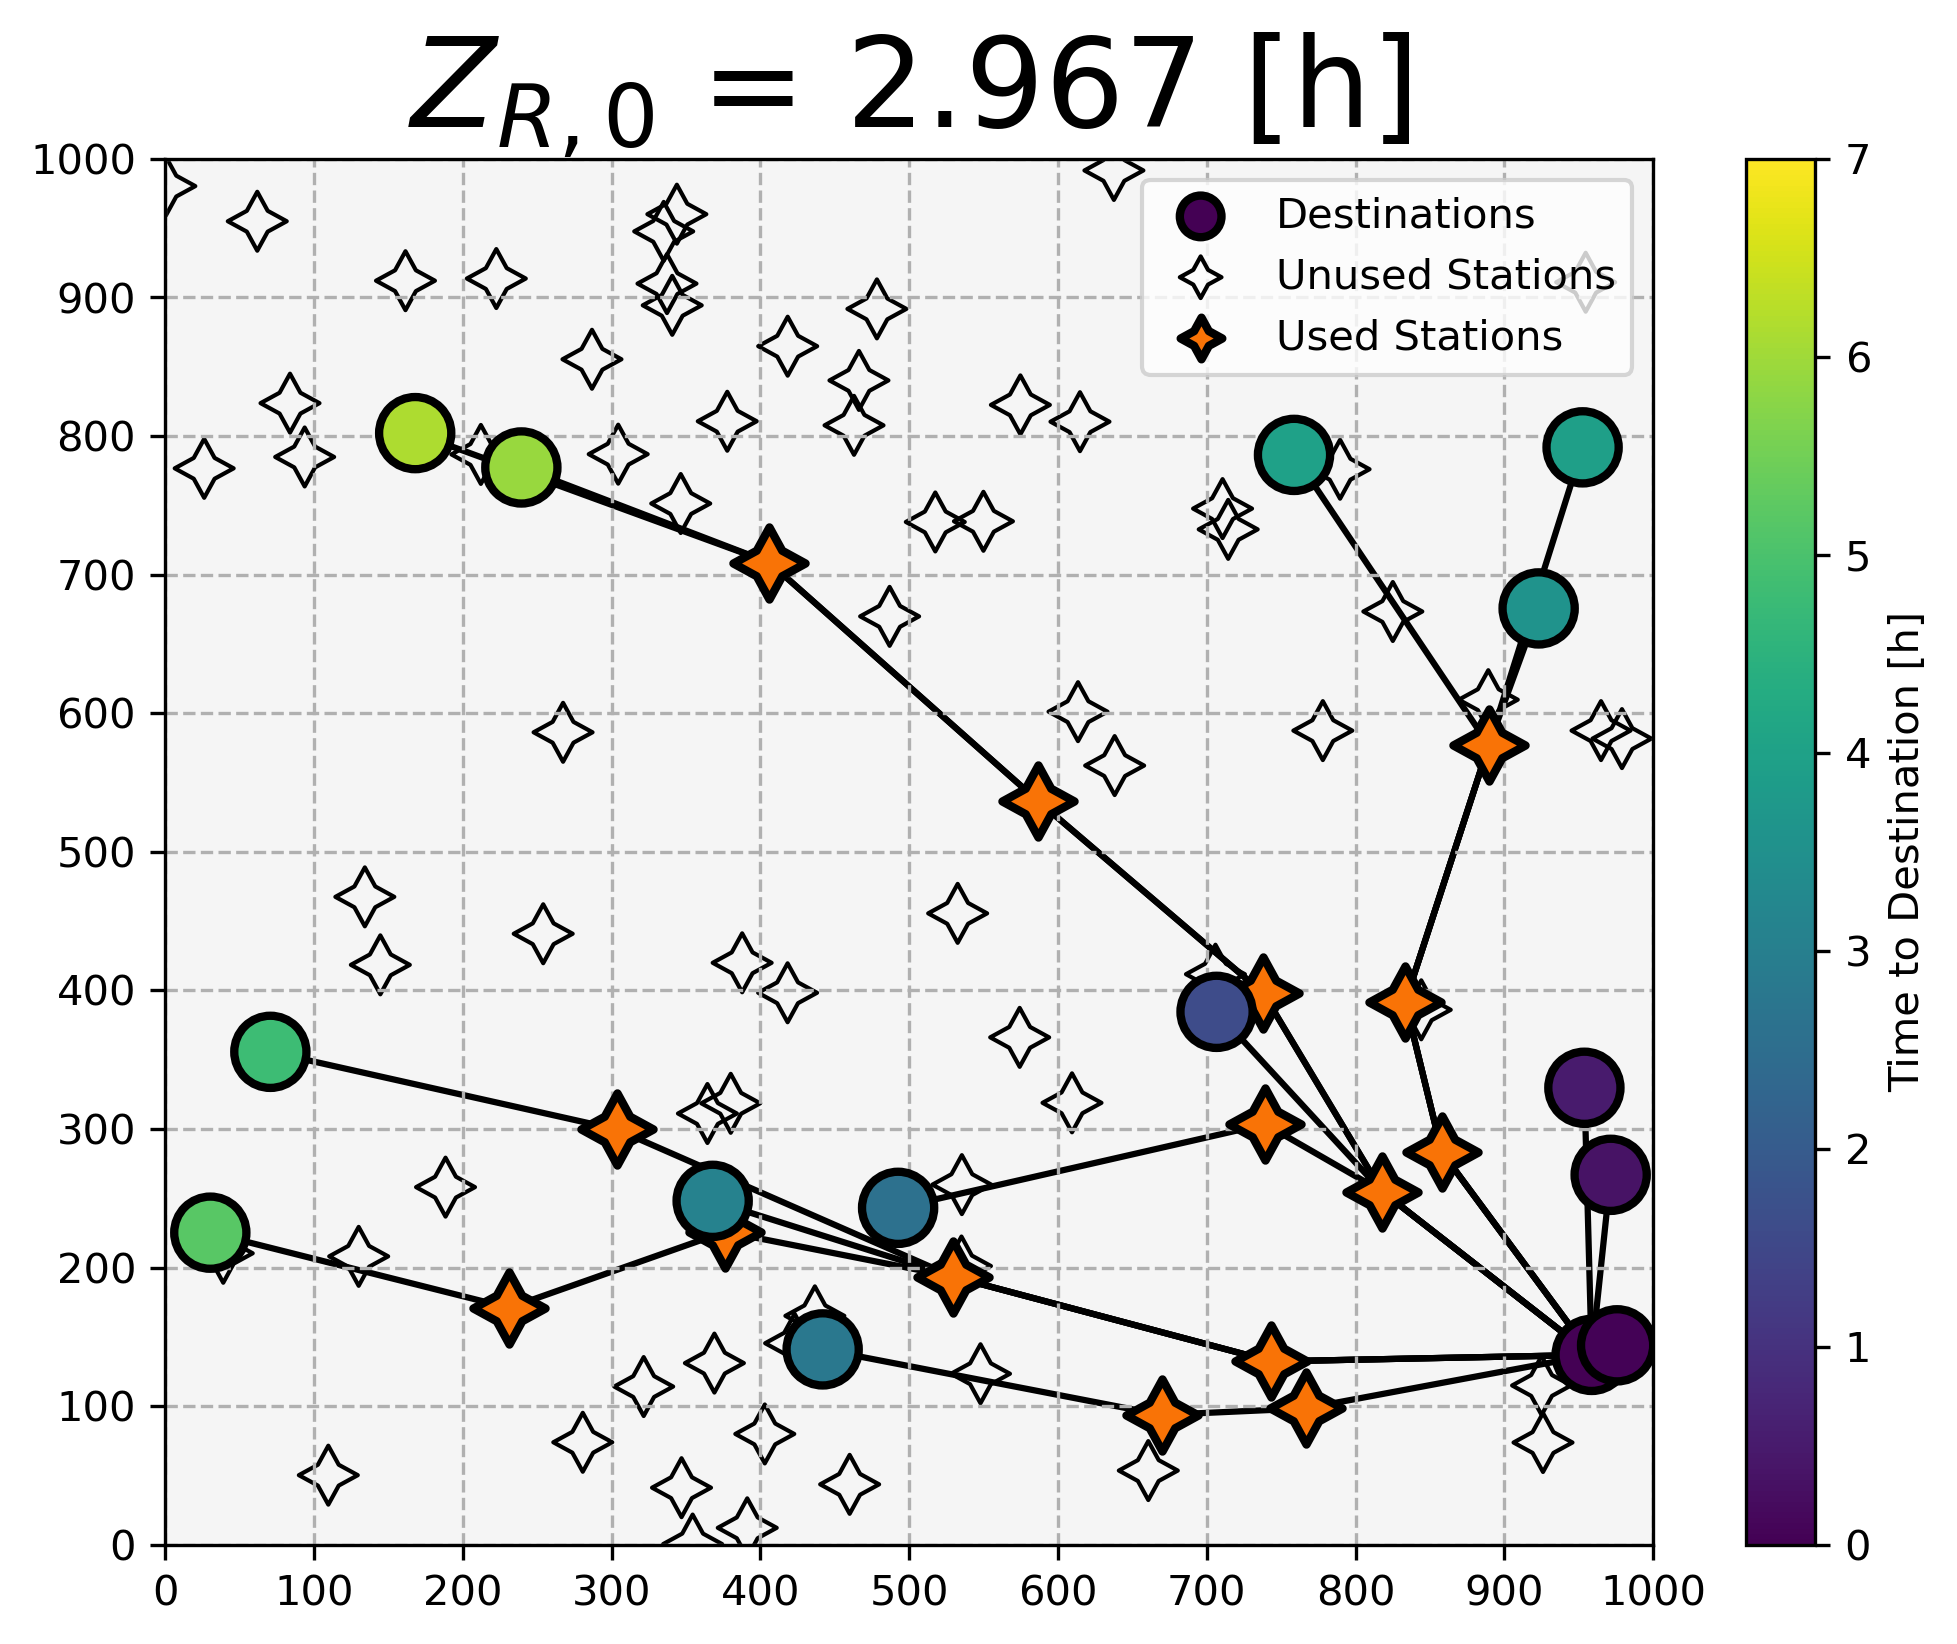
\includegraphics[width = \linewidth]{figs/random_example_high_reliability_aggressive_actual.png}
		\caption{High reliability, aggressive}
	\end{subfigure}%
	\begin{subfigure}[t]{.5\linewidth}
		\centering\captionsetup{width = .8\linewidth}
		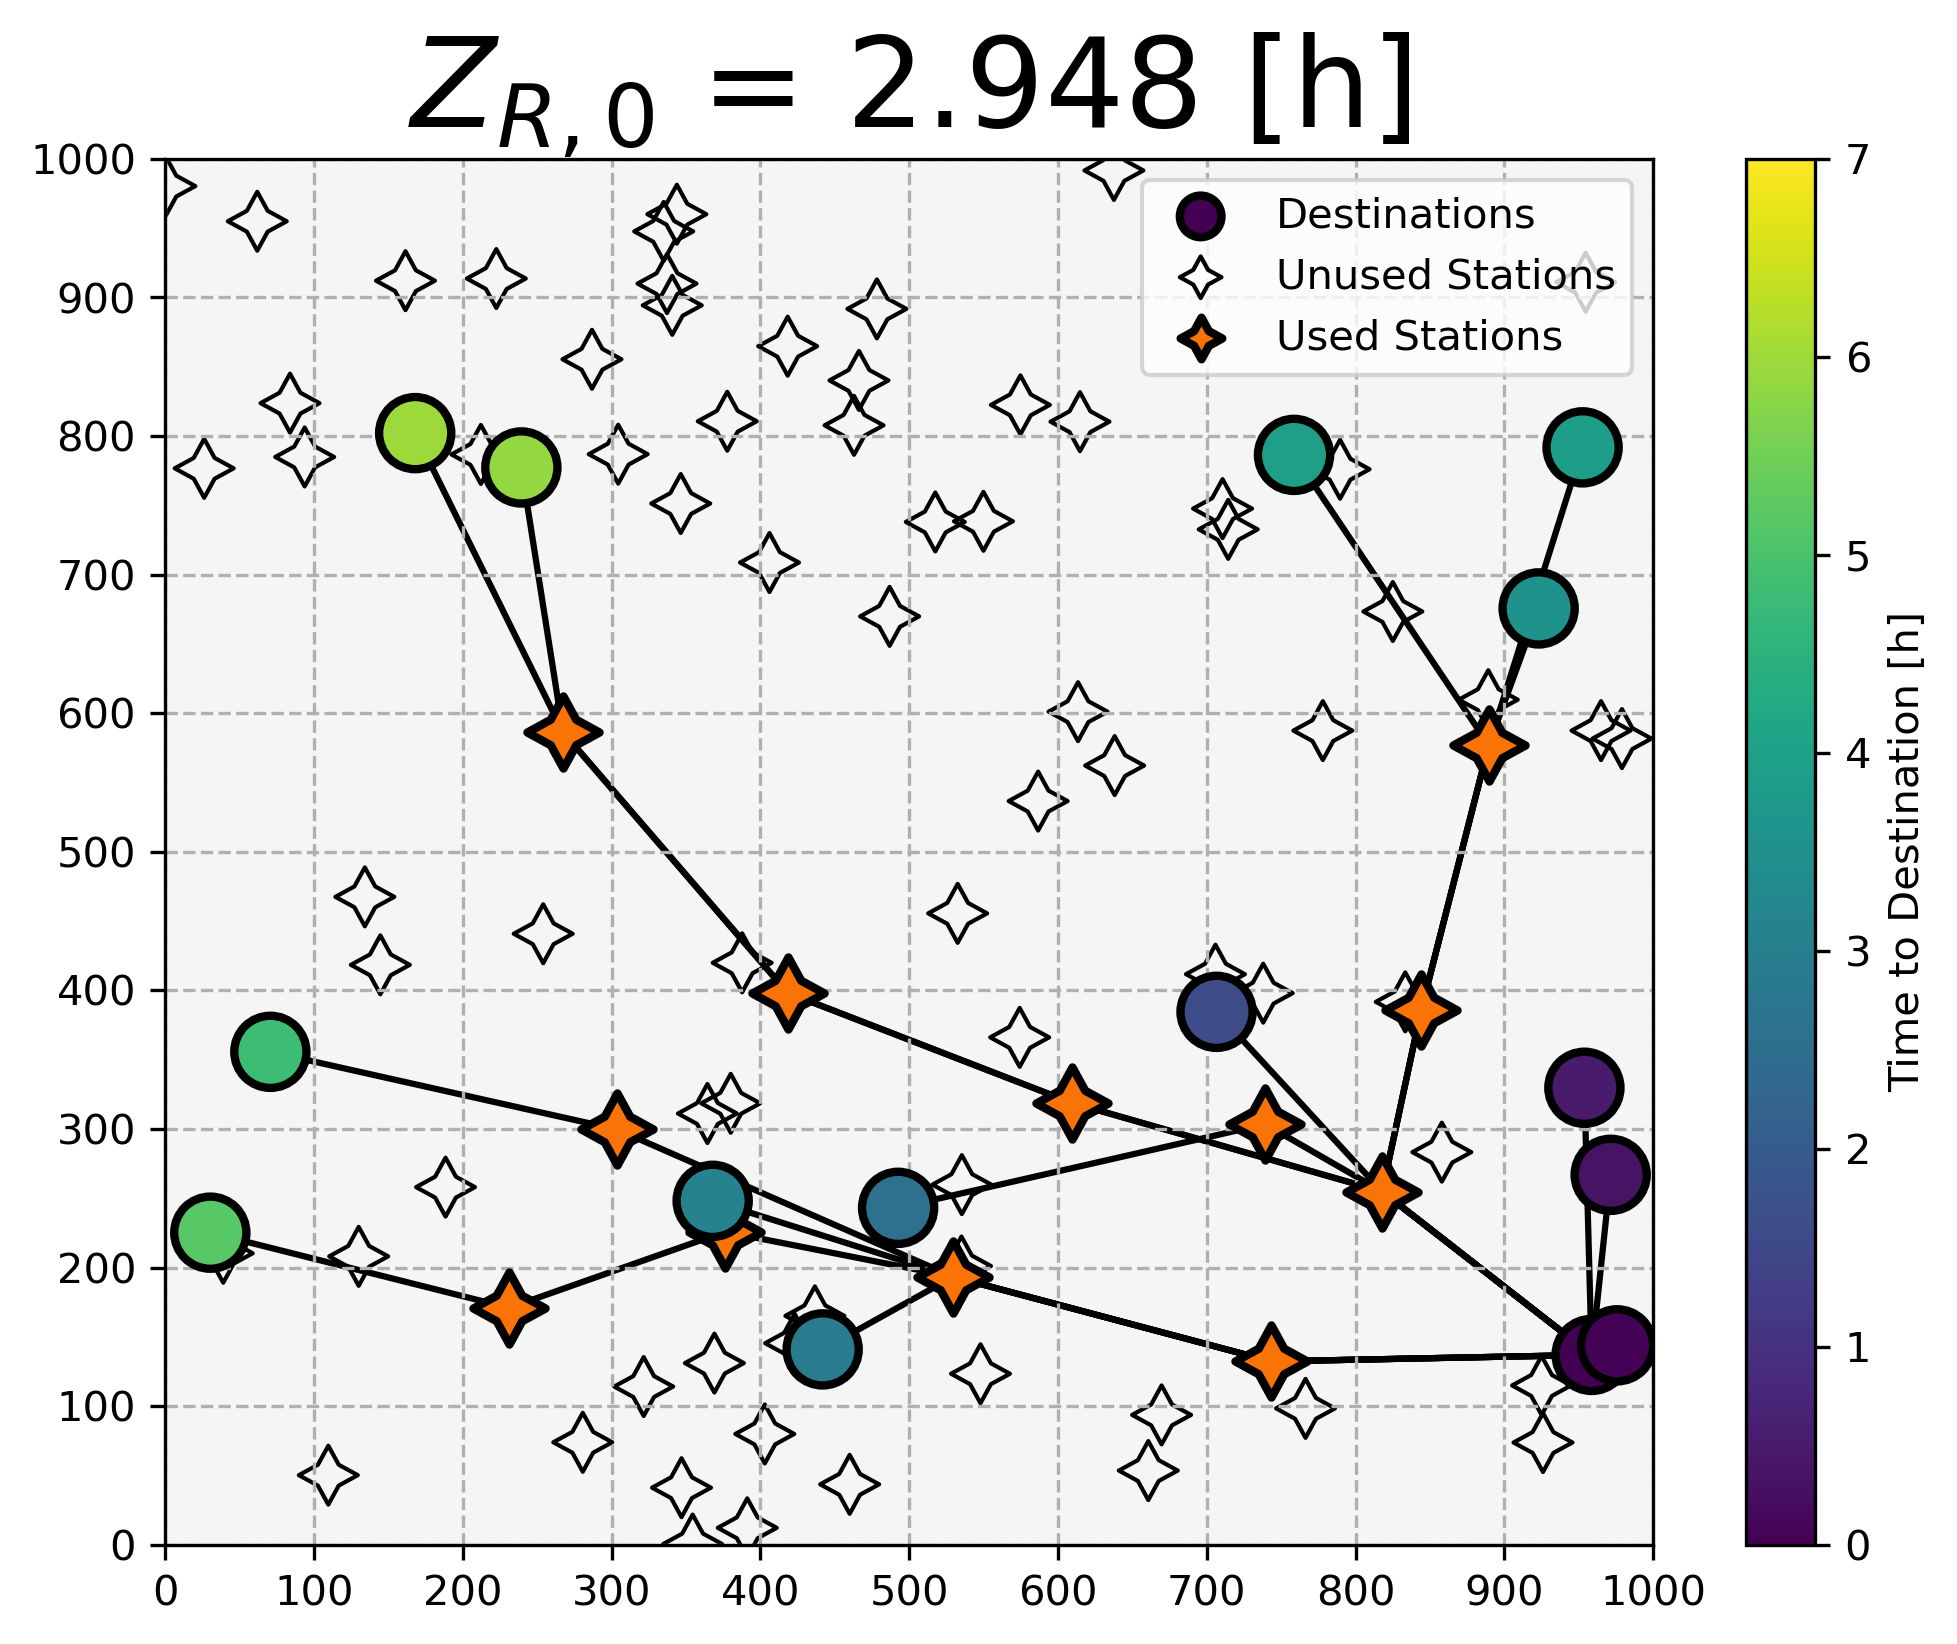
\includegraphics[width = \linewidth]{figs/random_example_high_reliability_cautious_actual.png}
		\caption{High reliability, cautious}
	\end{subfigure}
	\begin{subfigure}[t]{.5\linewidth}
		\centering\captionsetup{width = .8\linewidth}
		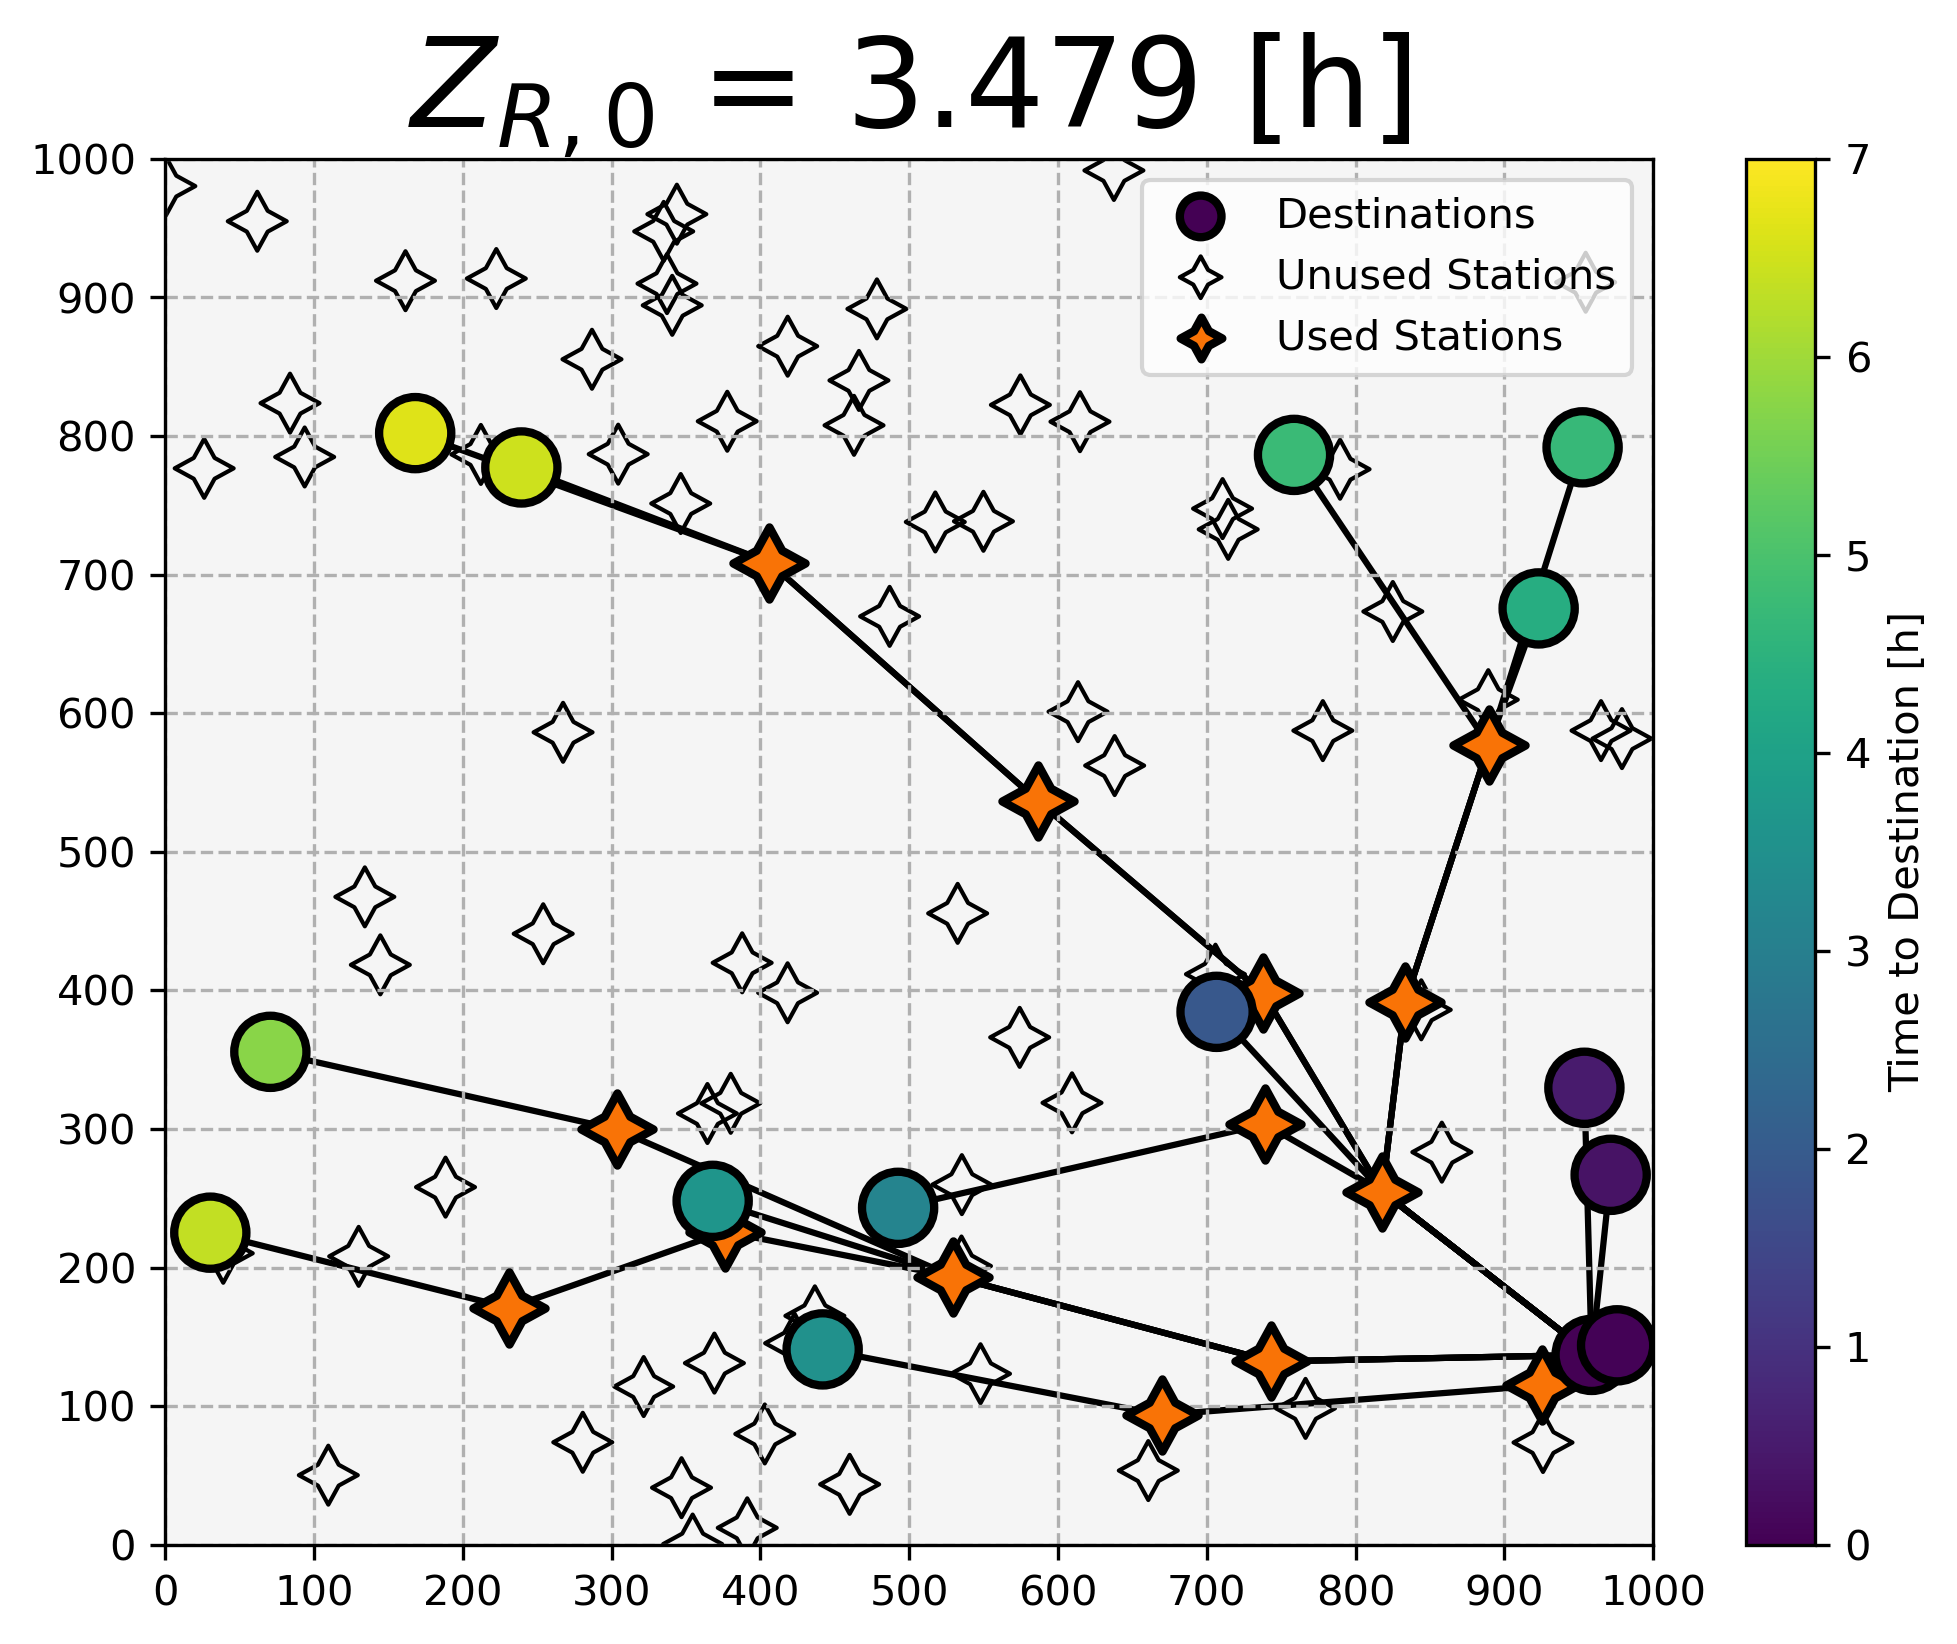
\includegraphics[width = \linewidth]{figs/random_example_low_reliability_aggressive_actual.png}
		\caption{Low reliability, aggressive}
	\end{subfigure}%
	\begin{subfigure}[t]{.5\linewidth}
		\centering\captionsetup{width = .8\linewidth}
		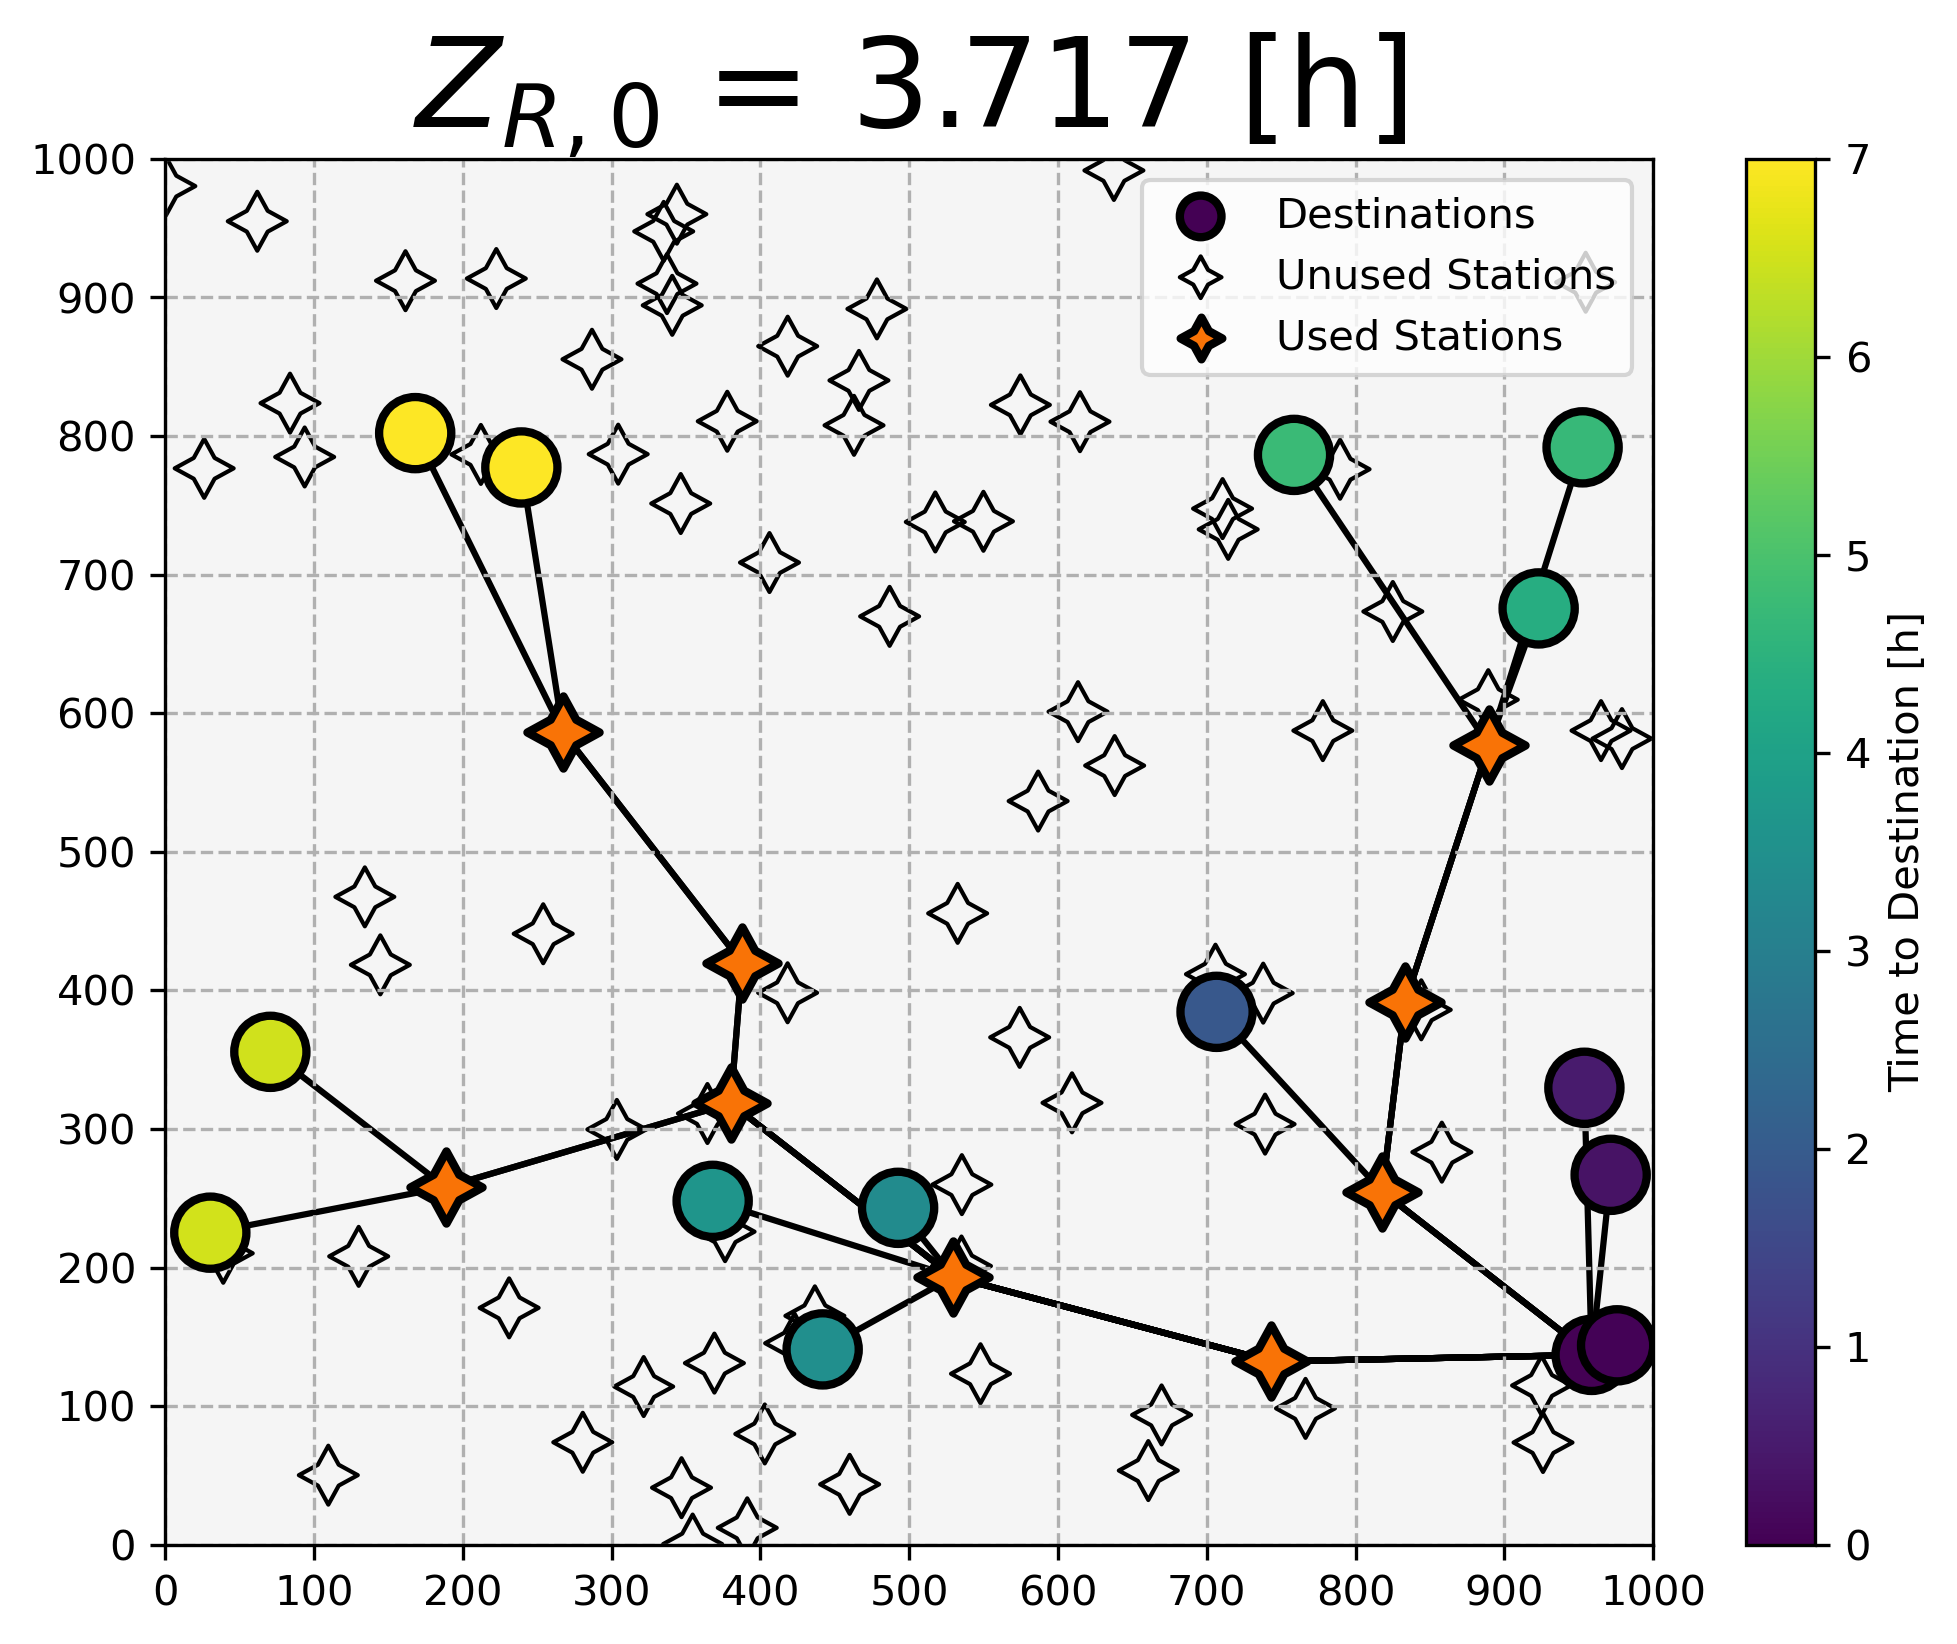
\includegraphics[width = \linewidth]{figs/random_example_low_reliability_cautious_actual.png}
		\caption{Low reliability, cautious}
	\end{subfigure}
	\caption{Neutral expectations of Specific Regional Impedance by risk attitude and port reliability.}
	\label{fig:perceived_srta_random_actual}
\end{figure}

The neutral expectations tell a different story. For the different levels of reliability, neutral expectations of impedance are similar for the routes selected by the aggressive and cautious drivers. The differences between biased and neutral perception are easy to understand. Both drivers selected routes based on a subset of the information and these routes are non-optimal when all information is considered. Drivers may adjust their priors over time but policy can only control the fundamentals. Thus, it is recommended to consider bias in route planning but neutral expectation in evaluation.

The composition of the routes taken by the drivers in the randomly generated example demonstrate an interesting dynamic as seen in Table \ref{tab:distances_redundancy}. As in-station redundancy is highly important in determining expected queuing times cautious drivers opt, increasingly for stations with higher in-station redundancy at the cost of taking less direct routes.

\begin{table}[H]
	\centering
	\caption{Average route distances and chargers per station utilized for example scenarios}
	\label{tab:distances_redundancy}
	\begin{tabular}{|C{\linewidth / 3}|C{\linewidth / 3}|C{\linewidth / 3}|}
		\hline Reliability & Risk-Attitude & Chargers per Station Utilized \\
		\hline High & Aggressive & 3.774 \\
		\hline High & Cautious & 4.258 \\
		\hline Low & Aggressive & 4.032 \\
		\hline Low & Cautious & 4.471 \\
		\hline
	\end{tabular}
\end{table}